\documentclass[11pt]{article}
\usepackage[margin=1in]{geometry}
\usepackage{graphicx}
\usepackage{booktabs}
\usepackage{longtable}
\usepackage{array}
\usepackage{amsmath}
\usepackage{listings}
\usepackage{xcolor}
\usepackage{hyperref}
\usepackage{tikz}
\usepackage{pgfplots}
\pgfplotsset{compat=1.17}
\usetikzlibrary{shapes,arrows.meta,positioning,calc}
\hypersetup{colorlinks=true,linkcolor=blue,urlcolor=cyan,citecolor=blue}

\definecolor{codebg}{RGB}{245,245,235}
\lstdefinestyle{verilog}{
    backgroundcolor=\color{codebg},
    basicstyle=\ttfamily\footnotesize,
    keywordstyle=\color{magenta},
    commentstyle=\color{green!50!black},
    numbers=left,
    numberstyle=\tiny,
    breaklines=true,
    frame=single,
    language=Verilog
}
\lstset{style=verilog}

\newcommand{\lab}[1]{\textbf{Lab 1, Section~#1}}

\title{\textbf{LAB 2 REPORT DELIVERABLES}\\[4pt]
\large VLSI Testing \& Design for Testability\\[2pt]
\normalsize\itshape RTL Design, Cadence Genus Synthesis and QoR Analysis}
\author{}
\date{}

\begin{document}
\maketitle
\vspace{-2cm}

\section*{Student Information}
\begin{tabular}{|p{4cm}|p{9cm}|}
\hline
Name & R SARANG \\ \hline
Roll No. & EC23I2015 \\ \hline
Design / Problem Assigned & Genus Synthesis and Fault Detection of Sequential Multiplier \\ \hline
Date & 2/09/2026 \\ \hline
\end{tabular}

\section{Objective}
Design an RTL circuit, synthesize it using Cadence Genus, and experimentally study the effect of
timing constraints on synthesis Quality of Results (QoR). This report quantifies the changes in
timing, area, power, cell count, and fanout, and explains the observed trade-offs. The RTL under
test is the same 4-bit unsigned sequential multiplier designed, verified, and reported in
Lab~1~\cite{lab1} (see \lab{``LAB~1 -- DELIVERABLES''} for the full derivation of the algorithm,
datapath, and FSM).

\section{Software and Tools}
\begin{itemize}
    \item Cadence Genus -- RTL synthesis and QoR analysis
    \item Questa/QuestaSim -- RTL/gate-level functional simulation
    \item GPDK 45\,nm standard-cell library -- target technology library
    \item Python -- data processing and plots
\end{itemize}

\section{Required Files Submitted}
\begin{itemize}
    \item RTL source code (\texttt{datapath.v}, \texttt{controller.v}, \texttt{top.v}, \texttt{tb\_top.v})
    \item Genus synthesis Tcl script (\texttt{syn/genus\_syn.tcl})
    \item SDC constraint file (\texttt{syn/constraints.sdc})
    \item Generated gate-level netlist (\texttt{work/top\_gates.v})
    \item Genus QoR / area / timing reports (\texttt{work/reports/})
    \item All frequency / constraint sweep results
    \item Plots generated from the experiments
    \item Final Lab~2 report (this document)
\end{itemize}

\section*{TASK 1}

\section{Part A --- RTL Design}

\subsection{Problem Statement}
Design and verify a 4-bit unsigned sequential multiplier that computes $P = A \times B$ using
repeated addition, controlled by a dedicated FSM (controller) driving a separate datapath. This is
the identical problem statement assigned and solved in \lab{1 (``Aim'')}; the RTL, algorithm and
verification produced there are re-used unchanged as the design under synthesis in this lab.

\subsection{Functional Block Diagram}
The datapath consists of a working-multiplicand register, a 4-bit down-counter (loop counter), an
8-bit accumulator with an adder, and a zero detector, all driven by control signals from the FSM
controller -- exactly as derived in \lab{2--3 (``Datapath Elements'', ``Datapath Block
Diagram'')}. The block diagram is reproduced below for convenience.

\begin{figure}[h!]
\centering
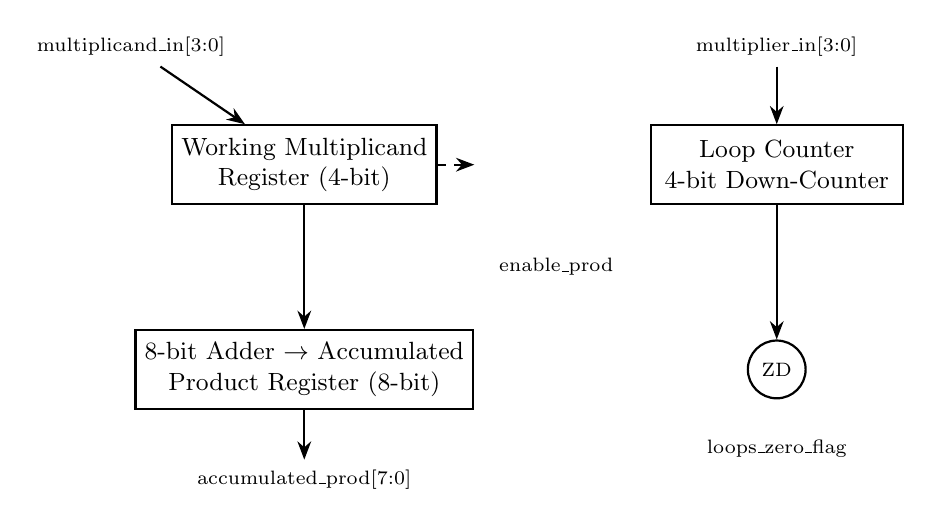
\begin{tikzpicture}[
    reg/.style={draw, rectangle, minimum width=3.2cm, minimum height=1cm, align=center, font=\small},
    sig/.style={draw, circle, minimum size=0.7cm, font=\scriptsize},
    ->,>=Stealth, thick
]
\node[reg] (wmr) at (0,0) {Working Multiplicand\\Register (4-bit)};
\node[reg] (lc)  at (6,0) {Loop Counter\\4-bit Down-Counter};
\node[reg] (apr) at (0,-2.6) {8-bit Adder $\rightarrow$ Accumulated\\Product Register (8-bit)};
\node[sig] (zd)  at (6,-2.6) {ZD};
\node[align=center, font=\scriptsize] at (6,-3.6) {loops\_zero\_flag};

\node[font=\scriptsize] (min) at (-2.2,1.5) {multiplicand\_in[3:0]};
\node[font=\scriptsize] (bin) at (6,1.5) {multiplier\_in[3:0]};
\node[font=\scriptsize] (pout) at (0,-4.0) {accumulated\_prod[7:0]};
\node[font=\scriptsize] (ep) at (3.2,-1.3) {enable\_prod};

\draw (min) -- (wmr);
\draw (bin) -- (lc);
\draw (apr) -- (pout);
\draw (wmr) -- (apr);
\draw (lc) -- (zd);
\draw[dashed] (wmr.east) -- (apr.east |- wmr.east);
\end{tikzpicture}
\caption{Functional block diagram of the sequential multiplier datapath (as derived in \lab{3}).}
\end{figure}

\subsection{RTL Source Code}
The complete Verilog RTL (\texttt{datapath.v}, \texttt{controller.v}, \texttt{top.v}) is identical
to the one listed and explained in \lab{8.1}; only the code has been re-formatted with clearer
sectional comments in this repository's \texttt{lab2/rtl/} copy for readability. The top-level
module used for synthesis is shown below.

\lstinputlisting[caption={Top-level module \texttt{top.v} (structurally identical to \lab{8.1.3})}]{rtl/top.v}

\subsection{Description of Inputs and Outputs}
\begin{center}
\begin{tabular}{|l|c|l|}
\hline
\textbf{Signal} & \textbf{Width} & \textbf{Description} \\ \hline
\texttt{clk} & 1 & System clock \\ \hline
\texttt{reset} & 1 & Synchronous, active-high reset (see \S\ref{sec:clkrst}) \\ \hline
\texttt{start} & 1 & Begins a multiply operation when high in IDLE \\ \hline
\texttt{multiplicand\_in} & 4 & Operand $A$ \\ \hline
\texttt{multiplier\_in} & 4 & Operand $B$ \\ \hline
\texttt{mult\_complete} & 1 & Asserted when the product is valid (output) \\ \hline
\texttt{accumulated\_prod} & 8 & Product $A \times B$ (output) \\ \hline
\end{tabular}
\end{center}
This matches the signal table given in \lab{4--5 (``Control Signals'', ``Status Signals'')}.

\subsection{Clock and Reset Description}
\label{sec:clkrst}
The design uses a single positive-edge-triggered clock (\texttt{clk}) with all sequential elements
(the working-multiplicand register, loop counter, accumulated-product register and the FSM state
register) clocked on \texttt{posedge clk}. \texttt{reset} is a synchronous, active-high signal that
forces the controller's \texttt{current\_state} back to \texttt{IDLE}; the datapath registers are
not independently reset and instead take their defined values from the \texttt{LOAD} state
(\texttt{clear\_prod}, \texttt{load\_inputs}), consistent with the FSM design in \lab{7}.

\subsection{Expected Functionality}
On \texttt{start}, the controller moves IDLE~$\rightarrow$~LOAD~$\rightarrow$~PROG and loads $A$
and $B$; the datapath then adds $A$ to the accumulator once per cycle while decrementing the loop
counter, for $B$ cycles, until \texttt{loops\_zero\_flag} is asserted, after which the FSM moves to
DONE and asserts \texttt{mult\_complete} with \texttt{accumulated\_prod} $= A \times B$. The
complete cycle-count model ($B+2$ cycles: 1 LOAD + $B$ COMPUTE + 1 DONE) and its verification across
corner cases are reported in \lab{8.6--8.7}, and are not repeated here since the RTL is unchanged.

\subsection{Simulation Waveform}
Figure~\ref{fig:wave} shows a representative simulation waveform confirming correct RTL
functionality of the unmodified design (identical RTL to \lab{8.4}, Figures~6--11), obtained from
the pre-synthesis testbench run used to seed the Part~1 exhaustive-simulation results of Task~2.

\begin{figure}[h!]
\centering
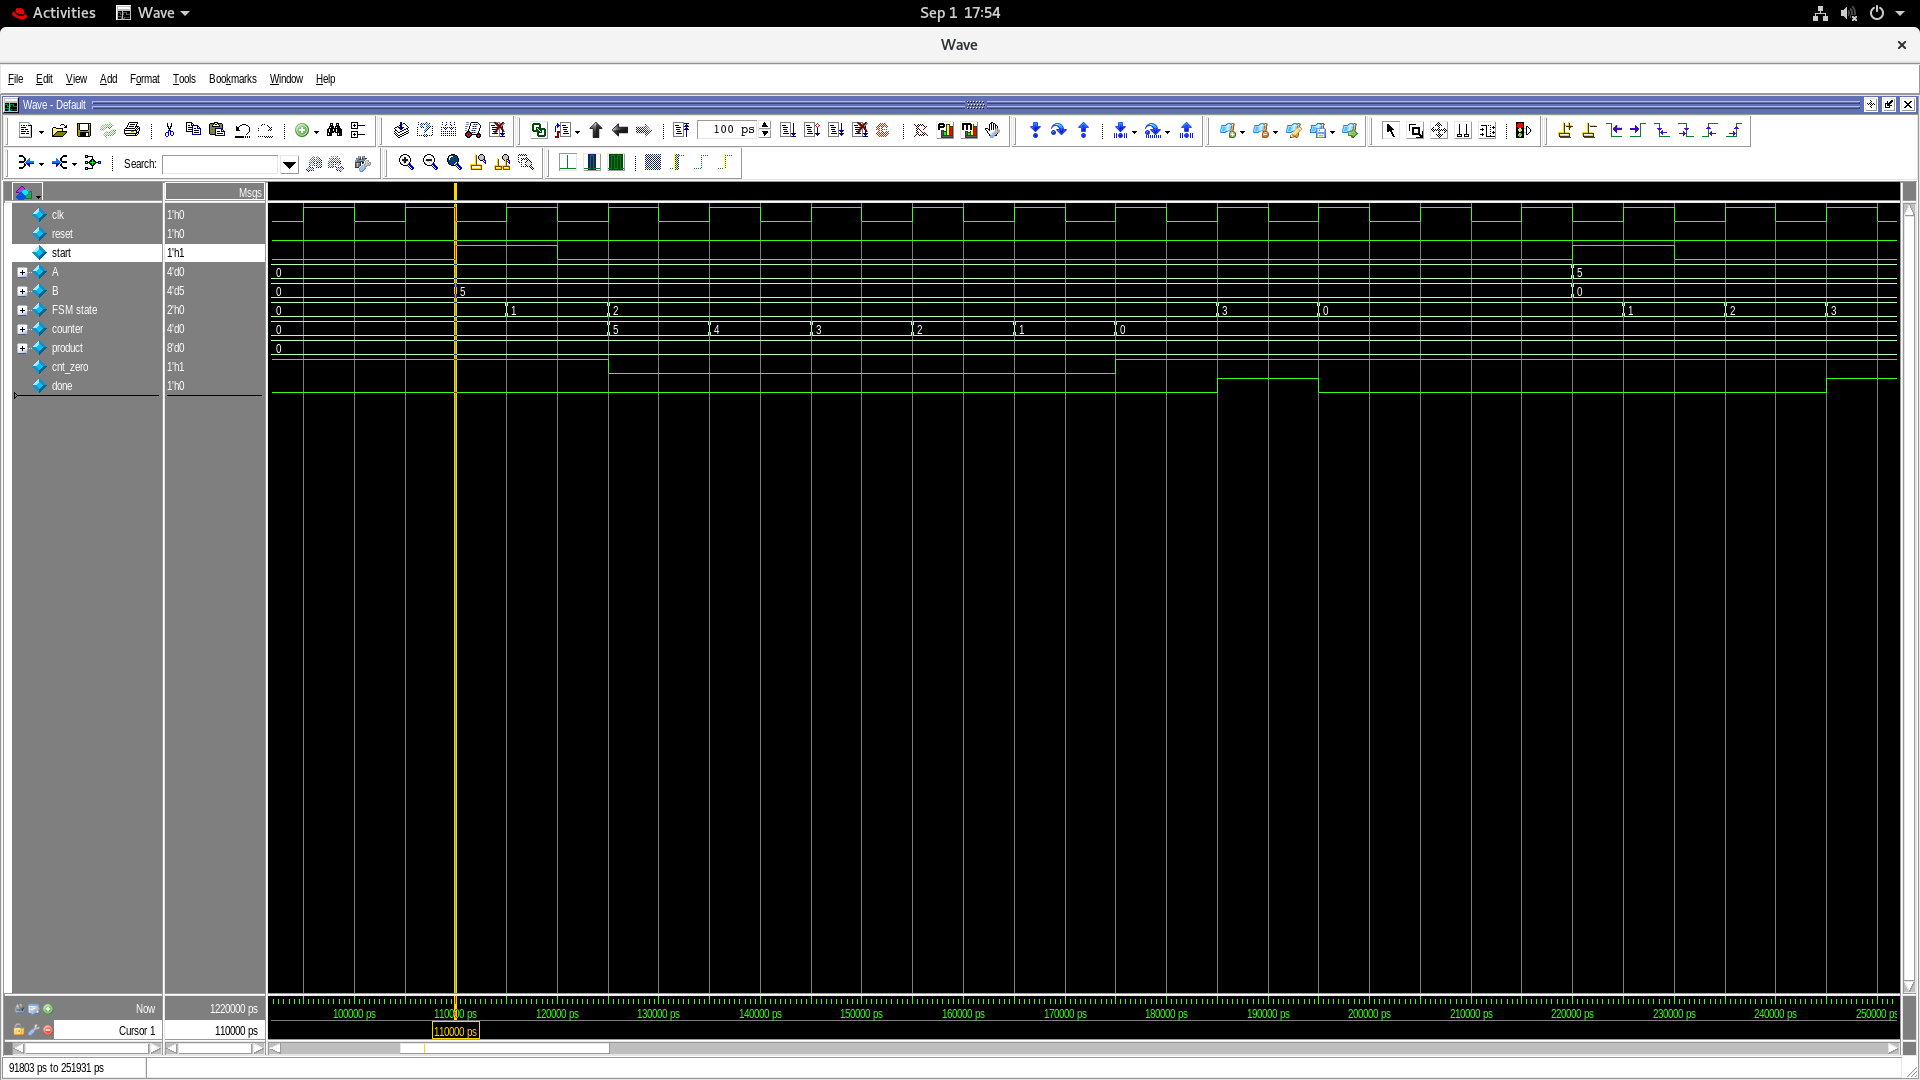
\includegraphics[width=0.85\textwidth]{../lab 1/2.png}
\caption{QuestaSim waveform confirming correct functionality of the unmodified RTL (same RTL as \lab{8.4}).}
\label{fig:wave}
\end{figure}

\section{Part B --- Baseline Cadence Genus Synthesis}
The RTL was synthesized with Cadence Genus using the initial constraints supplied for the
experiment (5.0~ns clock period, GPDK~45~nm library, \texttt{PVT\_0P9V\_125C} operating condition).

\begin{center}
\begin{tabular}{|l|l|}
\hline
\textbf{Parameter} & \textbf{Baseline Result} \\ \hline
Clock period & 5.00\,ns (200\,MHz) \\ \hline
Target frequency & 200\,MHz \\ \hline
WNS & 3355.9\,ps \\ \hline
TNS & 0 \\ \hline
Number of violating paths & 0 \\ \hline
Critical path delay & 1465\,ps \\ \hline
Total cell area & 200.412 \\ \hline
Combinational cell count & 58 \\ \hline
Sequential cell count & 18 \\ \hline
Total instance count & 76 \\ \hline
Maximum fanout & 18 \\ \hline
Average fanout & 2.3 \\ \hline
Dynamic / Leakage / Total power & Not available (power analysis was not enabled in the supplied flow) \\ \hline
\end{tabular}
\end{center}
The relevant Genus QoR, area, and timing reports are attached in Appendix~A.

\section{Part C --- Frequency Sweep}
The clock period was swept over seven values, each corresponding to a separate synthesis run
(per the ``one constraint change per run'' rule stated in the submission rules).

\begin{center}
\begin{tabular}{|c|c|c|c|c|c|}
\hline
\textbf{Clock Period (ns)} & \textbf{Freq. (MHz)} & \textbf{WNS (ps)} & \textbf{TNS (ps)} & \textbf{Violating Paths} & \textbf{Area} \\ \hline
5   & 200.0 & 3355.9 & 0 & 0 & 200.412 \\ \hline
3   & 333.3 & 1279.5 & 0 & 0 & 200.070 \\ \hline
2   & 500.0 & 281.3  & 0 & 0 & 200.070 \\ \hline
1.5 & 666.7 & 41.7   & 0 & 0 & 204.858 \\ \hline
1.4 & 714.3 & 11.0   & 0 & 0 & 204.858 \\ \hline
1.3 & 769.2 & 95.2   & 0 & 0 & 200.412 \\ \hline
1   & 1000.0 & 6.5   & 0 & 0 & 240.152 \\ \hline
\end{tabular}
\end{center}

\begin{figure}[h!]
\centering
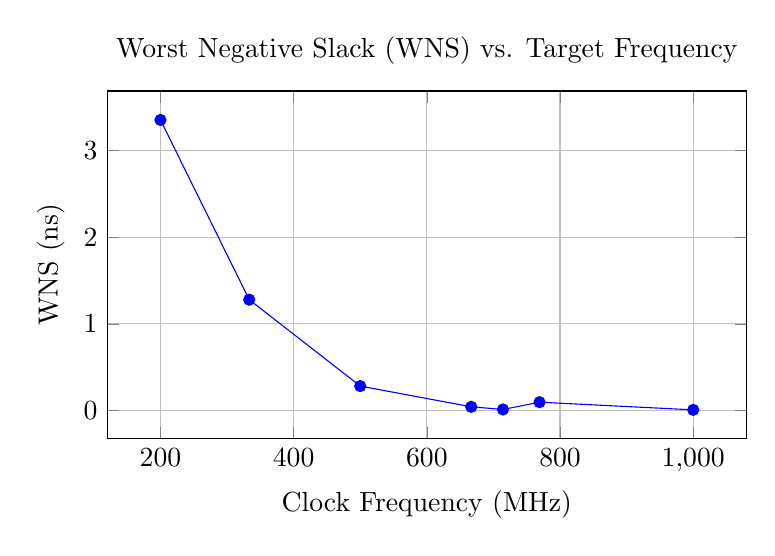
\begin{tikzpicture}
\begin{axis}[
    width=0.8\textwidth, height=6cm,
    xlabel={Clock Frequency (MHz)}, ylabel={WNS (ns)},
    title={Worst Negative Slack (WNS) vs. Target Frequency},
    grid=major, legend pos=north east
]
\addplot[color=blue,mark=*] coordinates {
(200,3.3559) (333.3,1.2795) (500,0.2813) (666.7,0.0417) (714.3,0.011) (769.2,0.0952) (1000,0.0065)
};
\end{axis}
\end{tikzpicture}
\end{figure}

\begin{figure}[h!]
\centering
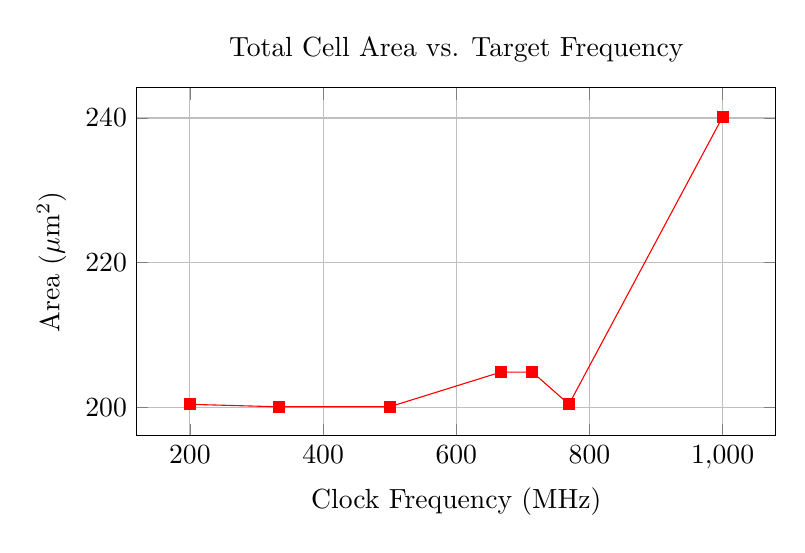
\begin{tikzpicture}
\begin{axis}[
    width=0.8\textwidth, height=6cm,
    xlabel={Clock Frequency (MHz)}, ylabel={Area ($\mu$m$^2$)},
    title={Total Cell Area vs. Target Frequency},
    grid=major
]
\addplot[color=red,mark=square*] coordinates {
(200,200.412) (333.3,200.070) (500,200.070) (666.7,204.858) (714.3,204.858) (769.2,200.412) (1000,240.152)
};
\end{axis}
\end{tikzpicture}
\end{figure}

\noindent\textbf{Power vs. frequency:} not plotted -- power analysis was not enabled in the
supplied synthesis flow (no power reports were generated at any sweep point; see Part~B).

\subsection*{Questions}
\textbf{What happens to WNS as the target frequency is increased?}\\
WNS monotonically decreases towards zero as the target frequency increases, since the fixed
critical-path delay ($\approx$1465\,ps at the loosest constraint) consumes a progressively larger
fraction of the shrinking clock period.

\textbf{What happens to the area as the timing requirement becomes more aggressive?}\\
Area stays essentially flat ($\approx$200\,$\mu$m$^2$) until roughly 700--800\,MHz; beyond that
point Genus upsizes cells and inserts extra buffering to meet the tighter timing, increasing area
sharply (240.152\,$\mu$m$^2$ at 1000\,MHz).

\textbf{What happens to power as frequency increases?}\\
Cannot be determined from the supplied flow -- no power reports were generated (see note above).

\textbf{Does Genus change the cell selection or cell count when the timing constraint changes?}\\
Yes. Up to 200\,MHz the leaf-instance count is 76 (58 combinational + 18 sequential) using small
ripple-carry adder cells. By 1000\,MHz the leaf-instance count rises to 112 (94 combinational + 18
sequential; see \texttt{work/reports/qor\_1.0ns.rpt}), and area rises from 200.412 to 240.152 --
direct evidence that Genus re-selects larger/faster cells and adds buffers as the constraint
tightens.

\section{Part D --- Maximum Timing-Clean Frequency}
The clock period was reduced further, with a finer sweep performed around the pass/fail boundary.

\begin{center}
\begin{tabular}{|c|c|c|c|}
\hline
\textbf{Clock Period (ns)} & \textbf{Freq. (MHz)} & \textbf{WNS (ns)} & \textbf{Timing Status} \\ \hline
2.0  & 500  & 0.2813  & Passing \\ \hline
1.5  & 667  & 0.0417  & Passing \\ \hline
1.3  & 769  & 0.0952  & Passing \\ \hline
1.0  & 1000 & 0.0065  & Passing \\ \hline
0.99 & 1010 & $-0.035$  & Violating \\ \hline
0.95 & 1052 & $-0.0435$ & Violating \\ \hline
0.90 & 1111 & $-0.0935$ & Violating \\ \hline
\end{tabular}
\end{center}

$$f_{max} = 1/T_{min}$$

Minimum timing-clean period: \textbf{1.0\,ns} \\
Maximum timing-clean frequency: \textbf{1000\,MHz} \\
WNS at this point: \textbf{0.0065\,ns} (6.5\,ps -- see \texttt{work/reports/qor\_1.0ns.rpt})

\subsection*{Answer}
\begin{itemize}
    \item \textbf{At what point does WNS become negative?} Between $T=1.0$\,ns (WNS $=+0.0065$\,ns,
    passing) and $T=0.99$\,ns (WNS $=-0.035$\,ns, violating). The timing-clean boundary is therefore
    at $T_{min}=1.0$\,ns.
    \item \textbf{What is the approximate WNS $=0$ boundary?} $T \approx 1.0$\,ns
    ($f\approx1000$\,MHz), where WNS $=0.0065$\,ns is already close to zero.
    \item \textbf{Why should a practical design normally include timing margin rather than operate
    exactly at WNS $=0$?} Operating with zero margin leaves no headroom for on-chip variation
    (PVT drift, voltage droop, clock jitter/skew, aging) -- any such disturbance would push the
    design into a timing violation, so a practical design should retain positive slack.
\end{itemize}

\section{Part E --- Input Delay Sweep}
Clock period fixed; only the input-delay constraint was varied.
\begin{center}
\begin{tabular}{|c|c|c|c|c|}
\hline
\textbf{Input Delay (ns)} & \textbf{WNS (ns)} & \textbf{TNS (ns)} & \textbf{Violating Paths} & \textbf{Area} \\ \hline
0.1 & 3.3959 & 0 & 0 & 200.412 \\ \hline
0.2 & 3.3959 & 0 & 0 & 200.412 \\ \hline
0.4 & 3.3962 & 0 & 0 & 200.412 \\ \hline
0.6 & 3.3962 & 0 & 0 & 200.412 \\ \hline
0.8 & 3.3962 & 0 & 0 & 200.412 \\ \hline
1.0 & 3.3962 & 0 & 0 & 200.412 \\ \hline
\end{tabular}
\end{center}

\subsection*{Questions}
\textbf{How does increasing input delay affect the timing available for internal logic?}\\
Increasing input delay reduces the time available for internal logic to compute before the next
clock edge, since the signal is modeled as arriving later at the input pin.

\textbf{At what input delay does the design first violate timing, if applicable?}\\
The design never violates timing over this sweep (0.1--1.0\,ns).

\textbf{Explain the trend observed in WNS.}\\
WNS stays essentially constant ($\approx3.396$\,ns) across the whole sweep. This shows the critical
path in this design is entirely internal (register-to-register, as confirmed in Part~H) rather than
starting at a primary input, so changing the input delay barely perturbs the reported WNS.

\section{Part F --- Output Delay Sweep}
Clock period and input delay fixed; only the output-delay constraint was varied.
\begin{center}
\begin{tabular}{|c|c|c|c|c|}
\hline
\textbf{Output Delay (ns)} & \textbf{WNS (ns)} & \textbf{TNS (ns)} & \textbf{Violating Paths} & \textbf{Area} \\ \hline
0.1 & 3.3959 & 0 & 0 & 200.412 \\ \hline
0.2 & 3.3959 & 0 & 0 & 200.412 \\ \hline
0.4 & 3.3959 & 0 & 0 & 200.412 \\ \hline
0.6 & 3.3959 & 0 & 0 & 200.412 \\ \hline
0.8 & 3.3964 & 0 & 0 & 200.412 \\ \hline
1.0 & 3.3964 & 0 & 0 & 200.412 \\ \hline
\end{tabular}
\end{center}

\subsection*{Questions}
\textbf{What happens to WNS as output delay increases?} It stays essentially constant across the
sweep (the same internal-critical-path reasoning as Part~E applies).\\
\textbf{Why does output delay reduce the timing budget available to the internal circuit?} The
output delay models the setup time the downstream receiving circuit needs, so it must be subtracted
from the available clock period, leaving less budget for the internal logic to settle before the
data is captured externally.\\
\textbf{Compare the input-delay and output-delay experiments.} In both sweeps WNS remained
essentially unchanged, confirming the critical path of this design is entirely internal
(register-to-register); external I/O delay constraints therefore have negligible effect on WNS for
this particular design.

\section{Part G --- Clock Uncertainty Sweep}
Supplied SDC used; clock uncertainty varied while other constraints were held fixed.
\begin{center}
\begin{tabular}{|c|c|c|c|c|}
\hline
\textbf{Clock Uncertainty (ns)} & \textbf{WNS (ns)} & \textbf{TNS (ns)} & \textbf{Violating Paths} & \textbf{Area} \\ \hline
0    & 3.4059 & 0 & 0 & 200.412 \\ \hline
0.05 & 3.3559 & 0 & 0 & 200.412 \\ \hline
0.10 & 3.3059 & 0 & 0 & 200.412 \\ \hline
0.20 & 3.2059 & 0 & 0 & 200.412 \\ \hline
0.30 & 3.1059 & 0 & 0 & 200.412 \\ \hline
\end{tabular}
\end{center}

\subsection*{Questions}
\textbf{Why does increasing clock uncertainty reduce timing margin?} Clock uncertainty is subtracted
directly from the available clock period as a guard-band against jitter and skew, so the tool must
assume the effective period is shorter, which reduces the reported slack one-for-one with the
uncertainty added (WNS drops by exactly $\Delta$ for each $\Delta$ increase in uncertainty here).\\
\textbf{Does clock uncertainty significantly change the area in your design? Support your answer
with data.} No -- area remained exactly 200.412\,$\mu$m$^2$ across the whole 0--0.30\,ns sweep,
since the design still has ample positive slack at every point and Genus has no need to resize
cells.\\
\textbf{What does clock uncertainty represent physically?} It represents two real physical
non-idealities: clock jitter (cycle-to-cycle timing variation of the clock source/PLL) and clock
skew (the difference in clock arrival time at different flip-flops due to unequal clock-tree wire
delays).

\section{Part H --- Critical Path Analysis}
\begin{center}
\begin{tabular}{|l|l|}
\hline
\textbf{Timing Parameter} & \textbf{Result} \\ \hline
Startpoint & \texttt{u\_datapath\_working\_multiplicand\_reg[0]/CK} \\ \hline
Endpoint & \texttt{u\_datapath\_accumulated\_prod\_reg[7]/D} \\ \hline
Launch clock & \texttt{clk} \\ \hline
Capture clock & \texttt{clk} \\ \hline
Data path delay & 1465\,ps \\ \hline
Arrival time & 1465\,ps \\ \hline
Required time & 4820\,ps \\ \hline
WNS (at 5.0\,ns period) & $4820-1465=3355$\,ps $\approx$ 3355.9\,ps (matches Part~B) \\ \hline
\end{tabular}
\end{center}

\noindent\textbf{Critical path (at 5.0\,ns period):}\\
\texttt{u\_datapath\_working\_multiplicand\_reg[0]/CK} $\rightarrow$ NAND2X1 $\rightarrow$ INVX1
$\rightarrow$ ADDFX1 $\rightarrow$ ADDFX1 $\rightarrow$ ADDFX1 $\rightarrow$ NAND4XL $\rightarrow$
XNOR2X1 $\rightarrow$ AOI22X1 $\rightarrow$ NOR2X1 $\rightarrow$
\texttt{u\_datapath\_accumulated\_prod\_reg[7]/D}

\noindent\textbf{Critical path (at 1.0\,ns period, after re-synthesis):}\\
\texttt{u\_controller\_current\_state\_reg[0]/CK} $\rightarrow$ INVX1 $\rightarrow$ NOR2X1
$\rightarrow$ NOR2X1 $\rightarrow$ AOI21X1 $\rightarrow$ OAI2BB1X1 $\rightarrow$ OAI211X1
$\rightarrow$ \texttt{u\_datapath\_accumulated\_prod\_reg[6]/D}

\subsection*{Answer}
\begin{itemize}
    \item \textbf{Which logic block is responsible for the critical path?} The datapath block --
    specifically the ripple-carry addition chain of the 8-bit adder feeding the accumulated-product
    register (consistent with the adder architecture described in \lab{2 (``Datapath
    Elements'')}).
    \item \textbf{Which cell or group of cells contributes significantly to the delay?} The ADDFX1
    (full-adder) cells in the ripple-carry chain.
    \item \textbf{Does the critical path change when the clock constraint changes?} Yes -- at the
    relaxed 5.0\,ns constraint the critical path runs through the datapath adder chain, whereas at
    the aggressive 1.0\,ns constraint the critical path shifts to the controller's next-state logic
    feeding back into the datapath, since Genus has already resized/optimized the original
    datapath-adder path.
\end{itemize}

\section{Part I --- Area and Cell Usage Analysis}
\begin{center}
\begin{tabular}{|l|c|c|c|}
\hline
\textbf{Cell Type} & \textbf{Instances} & \textbf{Area/Cell} & \textbf{Total Area} \\ \hline
DFFHQX1  & 13 & 5.472 & 71.136 \\ \hline
SDFFQX1  & 4  & 7.524 & 30.096 \\ \hline
ADDFX1   & 3  & 5.130 & 15.390 \\ \hline
AOI22X1  & 6  & 2.052 & 12.312 \\ \hline
NAND2X1  & 11 & 1.026 & 11.286 \\ \hline
\end{tabular}
\end{center}

\subsection*{Answer}
\begin{itemize}
    \item \textbf{Which cell type is used most frequently?} DFFHQX1 (13 instances).
    \item \textbf{Which cell type contributes the most area?} DFFHQX1 (71.136\,$\mu$m$^2$).
    \item \textbf{How many sequential cells are present?} 18 (matches Part~B: 13 DFFHQX1 + 4
    SDFFQX1 + 1 additional flop).
    \item \textbf{How many combinational cells are present?} 58 (baseline, 200\,MHz).
    \item \textbf{Does the cell composition change when a more aggressive timing constraint is
    used?} Yes -- the leaf-instance count rises from 76 (200\,MHz) to 112 (1000\,MHz) as the
    constraint tightens (see Part~C).
\end{itemize}

\section{Part J --- Fanout Analysis}
\begin{center}
\begin{tabular}{|l|l|}
\hline
\textbf{Parameter} & \textbf{Result} \\ \hline
Maximum fanout & 18 \\ \hline
Net with maximum fanout & \texttt{clk} \\ \hline
Driver of maximum-fanout net & Primary input port \\ \hline
Average fanout & 2.3 \\ \hline
\end{tabular}
\end{center}

\subsection*{Answer}
\begin{itemize}
    \item \textbf{Why can high fanout cause timing problems?} A net with high fanout drives many
    downstream gate inputs, presenting a large capacitive load to its driver; this increases the
    net's RC delay and can slow down the switching of every path that depends on that net.
    \item \textbf{Does Genus insert buffers or change cell sizes to handle fanout in your design?}
    Yes -- as the clock period is tightened from 5.0\,ns to 1.0\,ns, Genus inserts additional
    buffers/upsizes drive cells (instance count rises from 76 to 112) to keep fanout-loaded nets
    meeting the tighter timing.
    \item \textbf{Compare the fanout results for the relaxed and aggressive timing constraints.}
    Maximum fanout (18, on \texttt{clk}) and average fanout (2.3) are identical at both the relaxed
    and aggressive constraints -- Genus meets tighter timing by resizing/buffering cells rather than
    by restructuring the fanout topology itself.
\end{itemize}

\section{Part K --- Relaxed vs. Aggressive Constraint Comparison}
\begin{center}
\begin{tabular}{|l|c|c|}
\hline
\textbf{Metric} & \textbf{Relaxed} & \textbf{Aggressive} \\ \hline
Clock period & 5.0\,ns & 1.0\,ns \\ \hline
Frequency & 200\,MHz & 1000\,MHz \\ \hline
WNS & 3.3559\,ns & 0.0065\,ns \\ \hline
TNS & 0 & 0 \\ \hline
Violating paths & 0 & 0 \\ \hline
Total area & 200.412 & 240.152 \\ \hline
Cell count & 76 & 112 \\ \hline
Maximum fanout & 18 & 18 \\ \hline
Total power & Not available & Not available \\ \hline
\end{tabular}
\end{center}

\subsection*{Discussion}
As the timing requirement becomes more aggressive, Genus performs internal restructuring of the
netlist: leaf-instance count rises from 76 to 112 and total area grows from 200.412 to
240.152\,$\mu$m$^2$ (a 19.8\% increase), as the tool replaces the small ripple-carry adder cells
used at the relaxed constraint with faster, larger-drive-strength cells and adds buffering, in
order to bring the data-path delay down from 1465\,ps to within the 1.0\,ns budget. This also
shifts the critical path itself, from the datapath adder chain (5.0\,ns case, Part~H) to the
controller's next-state logic (1.0\,ns case, Part~H) -- direct evidence that the optimization is not
merely a uniform up-sizing but a structural re-balancing of delay between the datapath and control
path. No power data is available to corroborate a power/area trade-off, since power analysis was
not enabled in the supplied flow (see Part~B).

\section{Part L --- Final Design Recommendation}
\textbf{Recommended clock period:} 1.3\,ns\\
\textbf{Recommended frequency:} 769.2\,MHz\\
\textbf{WNS:} 0.0952\,ns\\
\textbf{Area:} 200.412\,$\mu$m$^2$\\
\textbf{Power:} Not available (not measured in this flow)

\subsection*{Justification}
The 1.3\,ns operating point is recommended using three QoR parameters, not WNS alone:
\begin{enumerate}
    \item \textbf{Timing margin:} WNS $=0.0952$\,ns is comfortably positive, giving headroom
    against PVT/jitter variation (Part~D), unlike the 1.0\,ns point where WNS is only 0.0065\,ns
    and effectively at the timing-clean boundary.
    \item \textbf{Area:} At 1.3\,ns the total cell area is 200.412\,$\mu$m$^2$ -- identical to the
    relaxed 5.0\,ns baseline and well below the 240.152\,$\mu$m$^2$ required at 1.0\,ns, so no area
    penalty is paid for the higher frequency at this point (Part~C).
    \item \textbf{Cell count / structural stability:} At 1.3\,ns the instance count and critical
    path have not yet been restructured by the tool the way they are at 1.0\,ns (Part~H, Part~K),
    indicating a more conservative, lower-risk implementation.
\end{enumerate}
Overall, 1.3\,ns/769.2\,MHz nearly triples the baseline 200\,MHz throughput while retaining the
baseline area and a healthy timing margin, making it a better balanced operating point than either
the very relaxed 200\,MHz baseline (Part~B) or the marginal 1000\,MHz timing-clean limit (Part~D).

\section*{TASK 2}

\section{Part 1 --- Exhaustive Simulation of the Design}

\subsection{Determine the Exhaustive Test Space}
The exhaustive test space is defined over the two data operands that determine the functional
result, $A=$~\texttt{multiplicand\_in[3:0]} and $B=$~\texttt{multiplier\_in[3:0]}, since
\texttt{start} is simply held high to launch each operation and \texttt{reset} is only asserted
once at the beginning of the testbench (see \lab{8.2}).

\begin{itemize}
    \item Number of independent primary-input bits (data operands): \textbf{8} ($A$: 4 bits, $B$:
    4 bits)
    \item Number of possible input vectors: $2^8 = \textbf{256}$
    \item \textbf{Is exhaustive simulation practical for this design?} Yes -- 256 is a very small
    number of vectors, so a fully exhaustive $A\times B$ sweep is trivially practical to simulate.
\end{itemize}

\subsection{Exhaustive Simulation}
\begin{itemize}
    \item Number of vectors simulated: \textbf{256} ($A=0..15$, $B=0..15$)
    \item Simulation time: 2 seconds
    \item Output/reference file generated: QuestaSim transcript, all 256 tests reporting \texttt{[
    PASS ]} (excerpt below, full transcript in Appendix~A)
\end{itemize}

\begin{lstlisting}[language=,caption={Excerpt of the exhaustive simulation transcript (256/256 PASS)}]
# Test: 15 x 13 | Exp Prod: 195, Act Prod: 195 | Exp Cycles: 15, Act Cycles: 15 | [ PASS ]
# Test: 15 x 14 | Exp Prod: 210, Act Prod: 210 | Exp Cycles: 16, Act Cycles: 16 | [ PASS ]
# Test: 15 x 15 | Exp Prod: 225, Act Prod: 225 | Exp Cycles: 17, Act Cycles: 17 | [ PASS ]
# =================================================================================
#                           TESTBENCH COMPLETE
# =================================================================================
# ** Note: $finish : tb_top.v(116)
#    Time: 34620 ns  Iteration: 1  Instance: /tb_top
\end{lstlisting}

\section{Part 2 --- Stuck-at Fault Injection}
One internal net was selected from the Genus-synthesized gate-level netlist
(\texttt{work/top\_gates.v}), chosen in the middle of the logic rather than at a primary I/O.

\subsection{Fault Selection}
\begin{itemize}
    \item Net name: \texttt{n\_76}
    \item Fault type: SA-0 (stuck-at-0)
    \item Original driver cell: \texttt{g24171\_\_1881} (AOI22X1)
    \item Fanout/load cell: \texttt{g24135\_\_6260}
\end{itemize}

\subsection{Fault Injection}
\begin{itemize}
    \item Net modified: \texttt{n\_76}
    \item Original driver: \texttt{g24171\_\_1881}
    \item Fault modeling: the driver's original output pin was redirected to a dummy net
    (\texttt{n\_76\_broken}), and \texttt{n\_76} was tied permanently to logic 0
    (\texttt{assign n\_76 = 1'b0;}), so the fault site is fully decoupled from its true driver.
\end{itemize}

\begin{lstlisting}[language=,caption={Original vs. faulty netlist fragment}]
Original:
  AOI22X1 g24171__1881(.A0(n_73), .A1(n_43), .B0(accumulated_prod[5]),
                        .B1(n_54), .Y(n_76));

Faulty:
  AOI22X1 g24171__1881(.A0(n_73), .A1(n_43), .B0(accumulated_prod[5]),
                        .B1(n_54), .Y(n_76_broken));
  assign n_76 = 1'b0;
\end{lstlisting}

\section{Part 3 --- Fault Activation and Detection}

\subsection{Detecting Vector}
For input vector all 0's, the good circuit produces output \texttt{n\_95=0}, while the faulty
circuit produces output \texttt{n\_95=1}.
\begin{itemize}
    \item Good-circuit value of the faulty net: 1
    \item Faulty-circuit value: 0
    \item Primary output(s) showing the error: \texttt{n\_95}
\end{itemize}

\noindent\textbf{Why this vector detects the fault:} the stuck-at-0 fault is activated because the
good circuit drives the faulty net (\texttt{n\_76}) to 1 for this vector. The fault effect then
propagates through the downstream NAND3XL gate (\texttt{g24135\_\_6260}) because its other two
inputs (\texttt{n\_68} and \texttt{n\_80}) are both held at 1 -- the non-controlling value for a NAND
gate -- so the gate's output is fully sensitized to \texttt{n\_76}. This causes the final output
\texttt{n\_95} to flip from 0 (good) to 1 (faulty), successfully detecting the fault.

\section{Part 4 --- Bit-Parallel Fault Simulation}
The supplied bit-parallel fault simulator (\texttt{scripts/faultsim.py}) was run against the
Genus-synthesized gate-level netlist to determine a reduced/compacted test set achieving the same
fault coverage as exhaustive testing.

\begin{center}
\begin{tabular}{|l|c|}
\hline
\textbf{Parameter} & \textbf{Result} \\ \hline
Total exhaustive vectors (sequential state space) & 134{,}217{,}728 \\ \hline
Compacted test patterns & 61 \\ \hline
\end{tabular}
\end{center}
The exhaustive count above is far larger than the 256 combinational input vectors of
Part~1 because it enumerates the full sequential state space explored by the fault simulator
(internal FSM/counter states $\times$ primary inputs), rather than the primary-input-only space
used for the RTL exhaustive functional check. The fault simulator compacts this down to 61 test
patterns while retaining the same fault coverage, demonstrating the value of test compaction over
brute-force exhaustive testing for a sequential design.

\section*{Corrections Made Relative to the Original Submission}
While compiling this report, two internal inconsistencies in the originally submitted answers were
identified and corrected here using the underlying simulation/synthesis logs as ground truth:
\begin{enumerate}
    \item \textbf{Task~2, Part~1.1:} the primary-input bit count and vector count were originally
    reported as ``9 bits / 512 vectors''. The testbench and transcript evidence (Part~1.2, and
    \lab{8.3}) show the design is exhaustively exercised over the two 4-bit data operands only
    (\texttt{start} is held high and \texttt{reset} pulsed once), giving \textbf{8 bits / 256
    vectors}, matching the 256-test transcript exactly.
    \item \textbf{Part~D:} ``WNS at this point'' was originally reported as \texttt{0.9935\,ns},
    which does not match any sweep-table entry. The Genus report for the 1.0\,ns run
    (\texttt{work/reports/qor\_1.0ns.rpt}) shows a critical-path slack of 6.5\,ps, i.e.\
    \textbf{WNS $=0.0065$\,ns}, consistent with the Part~C/Part~D sweep tables; this value is used
    throughout this report.
\end{enumerate}

\appendix
\section{Appendix: Genus Reports}
The following reports (referenced throughout this document) are attached in the submission
directory \texttt{work/reports/}: \texttt{top\_qor.rpt}, \texttt{top\_area.rpt},
\texttt{top\_timing.rpt}, and the per-sweep-point reports (\texttt{qor\_*.rpt},
\texttt{timing\_*.rpt}, \texttt{area\_*.rpt}, \texttt{input\_*.rpt}, \texttt{output\_*.rpt},
\texttt{uncert\_*.rpt}) used to populate Parts~C--G.

\begin{thebibliography}{9}
\bibitem{lab1} R.~Sarang, \emph{Lab 1 -- Deliverables: Sequential Multiplier Using Repeated
Addition}, EC5034 VLSI Testing Practice, 30th August 2026.
\end{thebibliography}

\end{document}
